\documentclass[twoside]{book}

% Packages required by doxygen
\usepackage{fixltx2e}
\usepackage{calc}
\usepackage{doxygen}
\usepackage[export]{adjustbox} % also loads graphicx
\usepackage{graphicx}
\usepackage[utf8]{inputenc}
\usepackage{makeidx}
\usepackage{multicol}
\usepackage{multirow}
\PassOptionsToPackage{warn}{textcomp}
\usepackage{textcomp}
\usepackage[nointegrals]{wasysym}
\usepackage[table]{xcolor}

% Font selection
\usepackage[T1]{fontenc}
\usepackage[scaled=.90]{helvet}
\usepackage{courier}
\usepackage{amssymb}
\usepackage{sectsty}
\renewcommand{\familydefault}{\sfdefault}
\allsectionsfont{%
  \fontseries{bc}\selectfont%
  \color{darkgray}%
}
\renewcommand{\DoxyLabelFont}{%
  \fontseries{bc}\selectfont%
  \color{darkgray}%
}
\newcommand{\+}{\discretionary{\mbox{\scriptsize$\hookleftarrow$}}{}{}}

% Page & text layout
\usepackage{geometry}
\geometry{%
  a4paper,%
  top=2.5cm,%
  bottom=2.5cm,%
  left=2.5cm,%
  right=2.5cm%
}
\tolerance=750
\hfuzz=15pt
\hbadness=750
\setlength{\emergencystretch}{15pt}
\setlength{\parindent}{0cm}
\setlength{\parskip}{3ex plus 2ex minus 2ex}
\makeatletter
\renewcommand{\paragraph}{%
  \@startsection{paragraph}{4}{0ex}{-1.0ex}{1.0ex}{%
    \normalfont\normalsize\bfseries\SS@parafont%
  }%
}
\renewcommand{\subparagraph}{%
  \@startsection{subparagraph}{5}{0ex}{-1.0ex}{1.0ex}{%
    \normalfont\normalsize\bfseries\SS@subparafont%
  }%
}
\makeatother

% Headers & footers
\usepackage{fancyhdr}
\pagestyle{fancyplain}
\fancyhead[LE]{\fancyplain{}{\bfseries\thepage}}
\fancyhead[CE]{\fancyplain{}{}}
\fancyhead[RE]{\fancyplain{}{\bfseries\leftmark}}
\fancyhead[LO]{\fancyplain{}{\bfseries\rightmark}}
\fancyhead[CO]{\fancyplain{}{}}
\fancyhead[RO]{\fancyplain{}{\bfseries\thepage}}
\fancyfoot[LE]{\fancyplain{}{}}
\fancyfoot[CE]{\fancyplain{}{}}
\fancyfoot[RE]{\fancyplain{}{\bfseries\scriptsize Generated by Doxygen }}
\fancyfoot[LO]{\fancyplain{}{\bfseries\scriptsize Generated by Doxygen }}
\fancyfoot[CO]{\fancyplain{}{}}
\fancyfoot[RO]{\fancyplain{}{}}
\renewcommand{\footrulewidth}{0.4pt}
\renewcommand{\chaptermark}[1]{%
  \markboth{#1}{}%
}
\renewcommand{\sectionmark}[1]{%
  \markright{\thesection\ #1}%
}

% Indices & bibliography
\usepackage{natbib}
\usepackage[titles]{tocloft}
\setcounter{tocdepth}{3}
\setcounter{secnumdepth}{5}
\makeindex

% Hyperlinks (required, but should be loaded last)
\usepackage{ifpdf}
\ifpdf
  \usepackage[pdftex,pagebackref=true]{hyperref}
\else
  \usepackage[ps2pdf,pagebackref=true]{hyperref}
\fi
\hypersetup{%
  colorlinks=true,%
  linkcolor=blue,%
  citecolor=blue,%
  unicode%
}

% Custom commands
\newcommand{\clearemptydoublepage}{%
  \newpage{\pagestyle{empty}\cleardoublepage}%
}

\usepackage{caption}
\captionsetup{labelsep=space,justification=centering,font={bf},singlelinecheck=off,skip=4pt,position=top}

%===== C O N T E N T S =====

\begin{document}

% Titlepage & ToC
\hypersetup{pageanchor=false,
             bookmarksnumbered=true,
             pdfencoding=unicode
            }
\pagenumbering{alph}
\begin{titlepage}
\vspace*{7cm}
\begin{center}%
{\Large Splendor \\[1ex]\large 1.\+0 }\\
\vspace*{1cm}
{\large Generated by Doxygen 1.8.13}\\
\end{center}
\end{titlepage}
\clearemptydoublepage
\pagenumbering{roman}
\tableofcontents
\clearemptydoublepage
\pagenumbering{arabic}
\hypersetup{pageanchor=true}

%--- Begin generated contents ---
\chapter{R\+E\+A\+D\+ME}
\label{md__r_e_a_d_m_e}
\Hypertarget{md__r_e_a_d_m_e}
\input{md__r_e_a_d_m_e}
\chapter{Namespace Index}
\section{Packages}
Here are the packages with brief descriptions (if available)\+:\begin{DoxyCompactList}
\item\contentsline{section}{\hyperlink{namespace_splendor}{Splendor} }{\pageref{namespace_splendor}}{}
\item\contentsline{section}{\hyperlink{namespace_splendor_1_1_properties}{Splendor.\+Properties} }{\pageref{namespace_splendor_1_1_properties}}{}
\end{DoxyCompactList}

\chapter{Hierarchical Index}
\section{Class Hierarchy}
This inheritance list is sorted roughly, but not completely, alphabetically\+:\begin{DoxyCompactList}
\item \contentsline{section}{Splendor.\+Card}{\pageref{class_splendor_1_1_card}}{}
\item \contentsline{section}{Splendor.\+Connection\+DB}{\pageref{class_splendor_1_1_connection_d_b}}{}
\item Form\begin{DoxyCompactList}
\item \contentsline{section}{Splendor.\+Ajouter\+Un\+Joueur}{\pageref{class_splendor_1_1_ajouter_un_joueur}}{}
\item \contentsline{section}{Splendor.\+frm\+Splendor}{\pageref{class_splendor_1_1frm_splendor}}{}
\end{DoxyCompactList}
\item \contentsline{section}{Splendor.\+Functions}{\pageref{class_splendor_1_1_functions}}{}
\item \contentsline{section}{Splendor.\+Player}{\pageref{class_splendor_1_1_player}}{}
\item \contentsline{section}{Splendor.\+Tools}{\pageref{class_splendor_1_1_tools}}{}
\end{DoxyCompactList}

\chapter{Class Index}
\section{Class List}
Here are the classes, structs, unions and interfaces with brief descriptions\+:\begin{DoxyCompactList}
\item\contentsline{section}{\hyperlink{class_splendor_1_1_card}{Splendor.\+Card} \\*Class \hyperlink{class_splendor_1_1_card}{Card} \+: attributes and methods to deal with a card }{\pageref{class_splendor_1_1_card}}{}
\item\contentsline{section}{\hyperlink{class_splendor_1_1_connection_d_b}{Splendor.\+Connection\+DB} \\*Contains methods and attributes to connect and deal with the database }{\pageref{class_splendor_1_1_connection_d_b}}{}
\item\contentsline{section}{\hyperlink{class_splendor_1_1frm_splendor}{Splendor.\+frm\+Splendor} \\*Manages the form that enables to play with the \hyperlink{namespace_splendor}{Splendor} }{\pageref{class_splendor_1_1frm_splendor}}{}
\item\contentsline{section}{\hyperlink{class_splendor_1_1_player}{Splendor.\+Player} \\*Class \hyperlink{class_splendor_1_1_player}{Player} \+: attributes and methods to deal with a player }{\pageref{class_splendor_1_1_player}}{}
\item\contentsline{section}{\hyperlink{class_splendor_1_1_tools}{Splendor.\+Tools} }{\pageref{class_splendor_1_1_tools}}{}
\end{DoxyCompactList}

\chapter{File Index}
\section{File List}
Here is a list of all documented files with brief descriptions\+:\begin{DoxyCompactList}
\item\contentsline{section}{Splendor/\hyperlink{_card_8cs}{Card.\+cs} \\*The model of card used in the game }{\pageref{_card_8cs}}{}
\item\contentsline{section}{Splendor/\hyperlink{_connection_d_b_8cs}{Connection\+D\+B.\+cs} \\*Set of methods related to DB connection }{\pageref{_connection_d_b_8cs}}{}
\item\contentsline{section}{Splendor/\hyperlink{frm_splendor_8cs}{frm\+Splendor.\+cs} \\*The famous \hyperlink{namespace_splendor}{Splendor} card game }{\pageref{frm_splendor_8cs}}{}
\item\contentsline{section}{Splendor/\hyperlink{_player_8cs}{Player.\+cs} \\*The model of player used in the game }{\pageref{_player_8cs}}{}
\item\contentsline{section}{Splendor/\hyperlink{_program_8cs}{Program.\+cs} \\*Entry point of the program }{\pageref{_program_8cs}}{}
\item\contentsline{section}{Splendor/\hyperlink{_tools_8cs}{Tools.\+cs} \\*Enumeration of the ressources of the game }{\pageref{_tools_8cs}}{}
\end{DoxyCompactList}

\chapter{Namespace Documentation}
\hypertarget{namespace_splendor}{}\section{Splendor Namespace Reference}
\label{namespace_splendor}\index{Splendor@{Splendor}}
\subsection*{Namespaces}
\begin{DoxyCompactItemize}
\end{DoxyCompactItemize}
\subsection*{Classes}
\begin{DoxyCompactItemize}
\item 
class \hyperlink{class_splendor_1_1_card}{Card}
\begin{DoxyCompactList}\small\item\em Class \hyperlink{class_splendor_1_1_card}{Card} \+: attributes and methods to deal with a card \end{DoxyCompactList}\item 
class \hyperlink{class_splendor_1_1_connection_d_b}{Connection\+DB}
\begin{DoxyCompactList}\small\item\em Contains methods and attributes to connect and deal with the database \end{DoxyCompactList}\item 
class \hyperlink{class_splendor_1_1frm_splendor}{frm\+Splendor}
\begin{DoxyCompactList}\small\item\em Manages the form that enables to play with the \hyperlink{namespace_splendor}{Splendor} \end{DoxyCompactList}\item 
class \hyperlink{class_splendor_1_1_player}{Player}
\begin{DoxyCompactList}\small\item\em Class \hyperlink{class_splendor_1_1_player}{Player} \+: attributes and methods to deal with a player \end{DoxyCompactList}\item 
class {\bfseries Program}
\item 
class \hyperlink{class_splendor_1_1_tools}{Tools}
\end{DoxyCompactItemize}
\subsection*{Enumerations}
\begin{DoxyCompactItemize}
\item 
\mbox{\Hypertarget{namespace_splendor_abc955fe800ad5f701f777df0a2a29dc2}\label{namespace_splendor_abc955fe800ad5f701f777df0a2a29dc2}} 
enum {\bfseries Ressources} \{ \newline
{\bfseries Or}, 
{\bfseries Rubis}, 
{\bfseries Emeraude}, 
{\bfseries Onyx}, 
\newline
{\bfseries Saphir}, 
{\bfseries Diamant}
 \}
\end{DoxyCompactItemize}

\hypertarget{namespace_splendor_1_1_properties}{}\section{Splendor.\+Properties Namespace Reference}
\label{namespace_splendor_1_1_properties}\index{Splendor.\+Properties@{Splendor.\+Properties}}
\subsection*{Classes}
\begin{DoxyCompactItemize}
\item 
class {\bfseries Resources}
\begin{DoxyCompactList}\small\item\em Une classe de ressource fortement typée destinée, entre autres, à la consultation des chaînes localisées. \end{DoxyCompactList}\item 
class {\bfseries Settings}
\end{DoxyCompactItemize}

\chapter{Class Documentation}
\hypertarget{class_splendor_1_1_card}{}\section{Splendor.\+Card Class Reference}
\label{class_splendor_1_1_card}\index{Splendor.\+Card@{Splendor.\+Card}}


Class \hyperlink{class_splendor_1_1_card}{Card} \+: attributes and methods to deal with a card  


\subsection*{Public Member Functions}
\begin{DoxyCompactItemize}
\item 
override string \hyperlink{class_splendor_1_1_card_a3403c28ee02b119ee5aae5bd10eee468}{To\+String} ()
\begin{DoxyCompactList}\small\item\em Displays information about the card \end{DoxyCompactList}\end{DoxyCompactItemize}
\subsection*{Properties}
\begin{DoxyCompactItemize}
\item 
Ressources \hyperlink{class_splendor_1_1_card_afcfaa7ea5072b3cd30c04adddc8dd5c7}{Ress}\hspace{0.3cm}{\ttfamily  \mbox{[}get, set\mbox{]}}
\begin{DoxyCompactList}\small\item\em The precious stone that the card gives \end{DoxyCompactList}\item 
int \hyperlink{class_splendor_1_1_card_a117119ceac083b7b7d39f11e5bbd7225}{Prestige\+Pt}\hspace{0.3cm}{\ttfamily  \mbox{[}get, set\mbox{]}}
\begin{DoxyCompactList}\small\item\em Number of prestige point of the card \end{DoxyCompactList}\item 
int \hyperlink{class_splendor_1_1_card_aadc9953aeb322c82e04fbd9b5a3b996d}{Level}\hspace{0.3cm}{\ttfamily  \mbox{[}get, set\mbox{]}}
\begin{DoxyCompactList}\small\item\em Level of the card \+: 1, 2 or 3 \end{DoxyCompactList}\item 
int \hyperlink{class_splendor_1_1_card_a1f2c57b133f35a3471ae86c9dc1727f6}{Id}\hspace{0.3cm}{\ttfamily  \mbox{[}get, set\mbox{]}}
\begin{DoxyCompactList}\small\item\em Id of the card in the database \end{DoxyCompactList}\item 
int \mbox{[}$\,$\mbox{]} \hyperlink{class_splendor_1_1_card_afee1b5ccf0c6745bdd9b7642a0158fae}{Price}\hspace{0.3cm}{\ttfamily  \mbox{[}get, set\mbox{]}}
\begin{DoxyCompactList}\small\item\em All the precious stones that are needed to buy the card \end{DoxyCompactList}\item 
bool \hyperlink{class_splendor_1_1_card_a3fb8ceaff1e5e581667aee29a8b70435}{Is\+Empty}\hspace{0.3cm}{\ttfamily  \mbox{[}get, set\mbox{]}}
\begin{DoxyCompactList}\small\item\em Tell if the card is void (new Card()) \end{DoxyCompactList}\end{DoxyCompactItemize}


\subsection{Detailed Description}
Class \hyperlink{class_splendor_1_1_card}{Card} \+: attributes and methods to deal with a card 



\subsection{Member Function Documentation}
\mbox{\Hypertarget{class_splendor_1_1_card_a3403c28ee02b119ee5aae5bd10eee468}\label{class_splendor_1_1_card_a3403c28ee02b119ee5aae5bd10eee468}} 
\index{Splendor\+::\+Card@{Splendor\+::\+Card}!To\+String@{To\+String}}
\index{To\+String@{To\+String}!Splendor\+::\+Card@{Splendor\+::\+Card}}
\subsubsection{\texorpdfstring{To\+String()}{ToString()}}
{\footnotesize\ttfamily override string Splendor.\+Card.\+To\+String (\begin{DoxyParamCaption}{ }\end{DoxyParamCaption})}



Displays information about the card 

\begin{DoxyReturn}{Returns}
A representation of the card in a string
\end{DoxyReturn}


\subsection{Property Documentation}
\mbox{\Hypertarget{class_splendor_1_1_card_a1f2c57b133f35a3471ae86c9dc1727f6}\label{class_splendor_1_1_card_a1f2c57b133f35a3471ae86c9dc1727f6}} 
\index{Splendor\+::\+Card@{Splendor\+::\+Card}!Id@{Id}}
\index{Id@{Id}!Splendor\+::\+Card@{Splendor\+::\+Card}}
\subsubsection{\texorpdfstring{Id}{Id}}
{\footnotesize\ttfamily int Splendor.\+Card.\+Id\hspace{0.3cm}{\ttfamily [get]}, {\ttfamily [set]}}



Id of the card in the database 

\mbox{\Hypertarget{class_splendor_1_1_card_a3fb8ceaff1e5e581667aee29a8b70435}\label{class_splendor_1_1_card_a3fb8ceaff1e5e581667aee29a8b70435}} 
\index{Splendor\+::\+Card@{Splendor\+::\+Card}!Is\+Empty@{Is\+Empty}}
\index{Is\+Empty@{Is\+Empty}!Splendor\+::\+Card@{Splendor\+::\+Card}}
\subsubsection{\texorpdfstring{Is\+Empty}{IsEmpty}}
{\footnotesize\ttfamily bool Splendor.\+Card.\+Is\+Empty\hspace{0.3cm}{\ttfamily [get]}, {\ttfamily [set]}}



Tell if the card is void (new Card()) 

\mbox{\Hypertarget{class_splendor_1_1_card_aadc9953aeb322c82e04fbd9b5a3b996d}\label{class_splendor_1_1_card_aadc9953aeb322c82e04fbd9b5a3b996d}} 
\index{Splendor\+::\+Card@{Splendor\+::\+Card}!Level@{Level}}
\index{Level@{Level}!Splendor\+::\+Card@{Splendor\+::\+Card}}
\subsubsection{\texorpdfstring{Level}{Level}}
{\footnotesize\ttfamily int Splendor.\+Card.\+Level\hspace{0.3cm}{\ttfamily [get]}, {\ttfamily [set]}}



Level of the card \+: 1, 2 or 3 

\mbox{\Hypertarget{class_splendor_1_1_card_a117119ceac083b7b7d39f11e5bbd7225}\label{class_splendor_1_1_card_a117119ceac083b7b7d39f11e5bbd7225}} 
\index{Splendor\+::\+Card@{Splendor\+::\+Card}!Prestige\+Pt@{Prestige\+Pt}}
\index{Prestige\+Pt@{Prestige\+Pt}!Splendor\+::\+Card@{Splendor\+::\+Card}}
\subsubsection{\texorpdfstring{Prestige\+Pt}{PrestigePt}}
{\footnotesize\ttfamily int Splendor.\+Card.\+Prestige\+Pt\hspace{0.3cm}{\ttfamily [get]}, {\ttfamily [set]}}



Number of prestige point of the card 

\mbox{\Hypertarget{class_splendor_1_1_card_afee1b5ccf0c6745bdd9b7642a0158fae}\label{class_splendor_1_1_card_afee1b5ccf0c6745bdd9b7642a0158fae}} 
\index{Splendor\+::\+Card@{Splendor\+::\+Card}!Price@{Price}}
\index{Price@{Price}!Splendor\+::\+Card@{Splendor\+::\+Card}}
\subsubsection{\texorpdfstring{Price}{Price}}
{\footnotesize\ttfamily int \mbox{[}$\,$\mbox{]} Splendor.\+Card.\+Price\hspace{0.3cm}{\ttfamily [get]}, {\ttfamily [set]}}



All the precious stones that are needed to buy the card 

\mbox{\Hypertarget{class_splendor_1_1_card_afcfaa7ea5072b3cd30c04adddc8dd5c7}\label{class_splendor_1_1_card_afcfaa7ea5072b3cd30c04adddc8dd5c7}} 
\index{Splendor\+::\+Card@{Splendor\+::\+Card}!Ress@{Ress}}
\index{Ress@{Ress}!Splendor\+::\+Card@{Splendor\+::\+Card}}
\subsubsection{\texorpdfstring{Ress}{Ress}}
{\footnotesize\ttfamily Ressources Splendor.\+Card.\+Ress\hspace{0.3cm}{\ttfamily [get]}, {\ttfamily [set]}}



The precious stone that the card gives 



The documentation for this class was generated from the following file\+:\begin{DoxyCompactItemize}
\item 
Splendor/\hyperlink{_card_8cs}{Card.\+cs}\end{DoxyCompactItemize}

\hypertarget{class_splendor_1_1_connection_d_b}{}\section{Splendor.\+Connection\+DB Class Reference}
\label{class_splendor_1_1_connection_d_b}\index{Splendor.\+Connection\+DB@{Splendor.\+Connection\+DB}}


Contains methods and attributes to connect and deal with the database  


\subsection*{Public Member Functions}
\begin{DoxyCompactItemize}
\item 
\hyperlink{class_splendor_1_1_connection_d_b_aaaa5c66d4f12702d36a76dd21beb62c4}{Connection\+DB} ()
\begin{DoxyCompactList}\small\item\em Constructor \+: Creates the connection to the database S\+Q\+Lite \end{DoxyCompactList}\item 
void \hyperlink{class_splendor_1_1_connection_d_b_a122fc944f46910732f429432c0f80ec3}{Add\+Player} (string player\+Name)
\begin{DoxyCompactList}\small\item\em Add a new player to the DB {\itshape player\+Name} Name of the player \end{DoxyCompactList}\item 
int \hyperlink{class_splendor_1_1_connection_d_b_a5731b9d427109c1d15db9665f290bf9a}{Get\+Number\+Of\+Players} ()
\begin{DoxyCompactList}\small\item\em Gets the number of players in the database \end{DoxyCompactList}\item 
string \hyperlink{class_splendor_1_1_connection_d_b_a7d715d5452049ad06f4a407fa5df151c}{Get\+Player\+Name} (int id)
\begin{DoxyCompactList}\small\item\em Get the name of the player according to his id \end{DoxyCompactList}\item 
List$<$ \hyperlink{class_splendor_1_1_card}{Card} $>$ \hyperlink{class_splendor_1_1_connection_d_b_aedda6930c46d2667248333ffca06882a}{Get\+List\+Card\+According\+To\+Level} (int level)
\begin{DoxyCompactList}\small\item\em Get the list of cards according to the level \end{DoxyCompactList}\item 
List$<$ \hyperlink{class_splendor_1_1_card}{Card} $>$ \hyperlink{class_splendor_1_1_connection_d_b_a020bd54ace4a6b36ccc8c1661d5322e7}{Get\+List\+Card} ()
\begin{DoxyCompactList}\small\item\em Get the list of all the cards \end{DoxyCompactList}\item 
\hyperlink{class_splendor_1_1_card}{Card} \hyperlink{class_splendor_1_1_connection_d_b_a1d7511e41b837b176737fd1b8d19f921}{Get\+Card\+By\+Id} (int id)
\begin{DoxyCompactList}\small\item\em Get card information with an id \end{DoxyCompactList}\item 
void \hyperlink{class_splendor_1_1_connection_d_b_a00d157ae467fdd310bf38626472175b6}{Remove\+Card\+By\+Id} (int id)
\begin{DoxyCompactList}\small\item\em Remove a card according a card with it\textquotesingle{}s id \end{DoxyCompactList}\end{DoxyCompactItemize}


\subsection{Detailed Description}
Contains methods and attributes to connect and deal with the database 



\subsection{Constructor \& Destructor Documentation}
\mbox{\Hypertarget{class_splendor_1_1_connection_d_b_aaaa5c66d4f12702d36a76dd21beb62c4}\label{class_splendor_1_1_connection_d_b_aaaa5c66d4f12702d36a76dd21beb62c4}} 
\index{Splendor\+::\+Connection\+DB@{Splendor\+::\+Connection\+DB}!Connection\+DB@{Connection\+DB}}
\index{Connection\+DB@{Connection\+DB}!Splendor\+::\+Connection\+DB@{Splendor\+::\+Connection\+DB}}
\subsubsection{\texorpdfstring{Connection\+D\+B()}{ConnectionDB()}}
{\footnotesize\ttfamily Splendor.\+Connection\+D\+B.\+Connection\+DB (\begin{DoxyParamCaption}{ }\end{DoxyParamCaption})}



Constructor \+: Creates the connection to the database S\+Q\+Lite 



\subsection{Member Function Documentation}
\mbox{\Hypertarget{class_splendor_1_1_connection_d_b_a122fc944f46910732f429432c0f80ec3}\label{class_splendor_1_1_connection_d_b_a122fc944f46910732f429432c0f80ec3}} 
\index{Splendor\+::\+Connection\+DB@{Splendor\+::\+Connection\+DB}!Add\+Player@{Add\+Player}}
\index{Add\+Player@{Add\+Player}!Splendor\+::\+Connection\+DB@{Splendor\+::\+Connection\+DB}}
\subsubsection{\texorpdfstring{Add\+Player()}{AddPlayer()}}
{\footnotesize\ttfamily void Splendor.\+Connection\+D\+B.\+Add\+Player (\begin{DoxyParamCaption}\item[{string}]{player\+Name }\end{DoxyParamCaption})}



Add a new player to the DB {\itshape player\+Name} Name of the player 

\mbox{\Hypertarget{class_splendor_1_1_connection_d_b_a1d7511e41b837b176737fd1b8d19f921}\label{class_splendor_1_1_connection_d_b_a1d7511e41b837b176737fd1b8d19f921}} 
\index{Splendor\+::\+Connection\+DB@{Splendor\+::\+Connection\+DB}!Get\+Card\+By\+Id@{Get\+Card\+By\+Id}}
\index{Get\+Card\+By\+Id@{Get\+Card\+By\+Id}!Splendor\+::\+Connection\+DB@{Splendor\+::\+Connection\+DB}}
\subsubsection{\texorpdfstring{Get\+Card\+By\+Id()}{GetCardById()}}
{\footnotesize\ttfamily \hyperlink{class_splendor_1_1_card}{Card} Splendor.\+Connection\+D\+B.\+Get\+Card\+By\+Id (\begin{DoxyParamCaption}\item[{int}]{id }\end{DoxyParamCaption})}



Get card information with an id 


\begin{DoxyParams}{Parameters}
{\em id} & \hyperlink{class_splendor_1_1_card}{Card}\textquotesingle{}s id\\
\hline
\end{DoxyParams}
\begin{DoxyReturn}{Returns}
\hyperlink{class_splendor_1_1_card}{Card} information
\end{DoxyReturn}
\mbox{\Hypertarget{class_splendor_1_1_connection_d_b_a020bd54ace4a6b36ccc8c1661d5322e7}\label{class_splendor_1_1_connection_d_b_a020bd54ace4a6b36ccc8c1661d5322e7}} 
\index{Splendor\+::\+Connection\+DB@{Splendor\+::\+Connection\+DB}!Get\+List\+Card@{Get\+List\+Card}}
\index{Get\+List\+Card@{Get\+List\+Card}!Splendor\+::\+Connection\+DB@{Splendor\+::\+Connection\+DB}}
\subsubsection{\texorpdfstring{Get\+List\+Card()}{GetListCard()}}
{\footnotesize\ttfamily List$<$\hyperlink{class_splendor_1_1_card}{Card}$>$ Splendor.\+Connection\+D\+B.\+Get\+List\+Card (\begin{DoxyParamCaption}{ }\end{DoxyParamCaption})}



Get the list of all the cards 

\begin{DoxyReturn}{Returns}
Cards list
\end{DoxyReturn}
\mbox{\Hypertarget{class_splendor_1_1_connection_d_b_aedda6930c46d2667248333ffca06882a}\label{class_splendor_1_1_connection_d_b_aedda6930c46d2667248333ffca06882a}} 
\index{Splendor\+::\+Connection\+DB@{Splendor\+::\+Connection\+DB}!Get\+List\+Card\+According\+To\+Level@{Get\+List\+Card\+According\+To\+Level}}
\index{Get\+List\+Card\+According\+To\+Level@{Get\+List\+Card\+According\+To\+Level}!Splendor\+::\+Connection\+DB@{Splendor\+::\+Connection\+DB}}
\subsubsection{\texorpdfstring{Get\+List\+Card\+According\+To\+Level()}{GetListCardAccordingToLevel()}}
{\footnotesize\ttfamily List$<$\hyperlink{class_splendor_1_1_card}{Card}$>$ Splendor.\+Connection\+D\+B.\+Get\+List\+Card\+According\+To\+Level (\begin{DoxyParamCaption}\item[{int}]{level }\end{DoxyParamCaption})}



Get the list of cards according to the level 


\begin{DoxyParams}{Parameters}
{\em level} & card\textquotesingle{}s level\\
\hline
\end{DoxyParams}
\begin{DoxyReturn}{Returns}
Cards list
\end{DoxyReturn}
\mbox{\Hypertarget{class_splendor_1_1_connection_d_b_a5731b9d427109c1d15db9665f290bf9a}\label{class_splendor_1_1_connection_d_b_a5731b9d427109c1d15db9665f290bf9a}} 
\index{Splendor\+::\+Connection\+DB@{Splendor\+::\+Connection\+DB}!Get\+Number\+Of\+Players@{Get\+Number\+Of\+Players}}
\index{Get\+Number\+Of\+Players@{Get\+Number\+Of\+Players}!Splendor\+::\+Connection\+DB@{Splendor\+::\+Connection\+DB}}
\subsubsection{\texorpdfstring{Get\+Number\+Of\+Players()}{GetNumberOfPlayers()}}
{\footnotesize\ttfamily int Splendor.\+Connection\+D\+B.\+Get\+Number\+Of\+Players (\begin{DoxyParamCaption}{ }\end{DoxyParamCaption})}



Gets the number of players in the database 

\begin{DoxyReturn}{Returns}
The number of players
\end{DoxyReturn}
\mbox{\Hypertarget{class_splendor_1_1_connection_d_b_a7d715d5452049ad06f4a407fa5df151c}\label{class_splendor_1_1_connection_d_b_a7d715d5452049ad06f4a407fa5df151c}} 
\index{Splendor\+::\+Connection\+DB@{Splendor\+::\+Connection\+DB}!Get\+Player\+Name@{Get\+Player\+Name}}
\index{Get\+Player\+Name@{Get\+Player\+Name}!Splendor\+::\+Connection\+DB@{Splendor\+::\+Connection\+DB}}
\subsubsection{\texorpdfstring{Get\+Player\+Name()}{GetPlayerName()}}
{\footnotesize\ttfamily string Splendor.\+Connection\+D\+B.\+Get\+Player\+Name (\begin{DoxyParamCaption}\item[{int}]{id }\end{DoxyParamCaption})}



Get the name of the player according to his id 


\begin{DoxyParams}{Parameters}
{\em id} & Id of the player\\
\hline
\end{DoxyParams}
\begin{DoxyReturn}{Returns}
\hyperlink{class_splendor_1_1_player}{Player} name
\end{DoxyReturn}
\mbox{\Hypertarget{class_splendor_1_1_connection_d_b_a00d157ae467fdd310bf38626472175b6}\label{class_splendor_1_1_connection_d_b_a00d157ae467fdd310bf38626472175b6}} 
\index{Splendor\+::\+Connection\+DB@{Splendor\+::\+Connection\+DB}!Remove\+Card\+By\+Id@{Remove\+Card\+By\+Id}}
\index{Remove\+Card\+By\+Id@{Remove\+Card\+By\+Id}!Splendor\+::\+Connection\+DB@{Splendor\+::\+Connection\+DB}}
\subsubsection{\texorpdfstring{Remove\+Card\+By\+Id()}{RemoveCardById()}}
{\footnotesize\ttfamily void Splendor.\+Connection\+D\+B.\+Remove\+Card\+By\+Id (\begin{DoxyParamCaption}\item[{int}]{id }\end{DoxyParamCaption})}



Remove a card according a card with it\textquotesingle{}s id 


\begin{DoxyParams}{Parameters}
{\em id} & \\
\hline
\end{DoxyParams}


The documentation for this class was generated from the following file\+:\begin{DoxyCompactItemize}
\item 
Splendor/\hyperlink{_connection_d_b_8cs}{Connection\+D\+B.\+cs}\end{DoxyCompactItemize}

\hypertarget{class_splendor_1_1frm_splendor}{}\section{Splendor.\+frm\+Splendor Class Reference}
\label{class_splendor_1_1frm_splendor}\index{Splendor.\+frm\+Splendor@{Splendor.\+frm\+Splendor}}


manages the form that enables to play with the \hyperlink{namespace_splendor}{Splendor}  


Inheritance diagram for Splendor.\+frm\+Splendor\+:\begin{figure}[H]
\begin{center}
\leavevmode
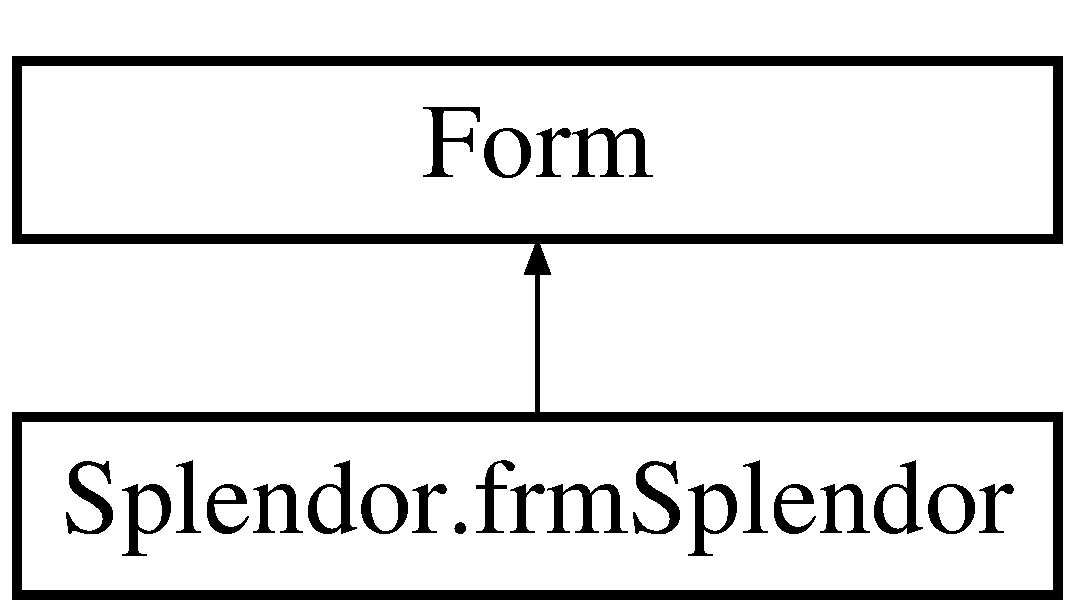
\includegraphics[height=2.000000cm]{class_splendor_1_1frm_splendor}
\end{center}
\end{figure}
\subsection*{Public Member Functions}
\begin{DoxyCompactItemize}
\item 
\hyperlink{class_splendor_1_1frm_splendor_ad9c938893d23192acb1996053e3ea87b}{frm\+Splendor} ()
\begin{DoxyCompactList}\small\item\em constructor \end{DoxyCompactList}\end{DoxyCompactItemize}
\subsection*{Protected Member Functions}
\begin{DoxyCompactItemize}
\item 
override void \hyperlink{class_splendor_1_1frm_splendor_a749f4f1d67c78e74aa1a55aa6fdd754b}{Dispose} (bool disposing)
\begin{DoxyCompactList}\small\item\em Nettoyage des ressources utilisées. \end{DoxyCompactList}\end{DoxyCompactItemize}


\subsection{Detailed Description}
manages the form that enables to play with the \hyperlink{namespace_splendor}{Splendor} 



\subsection{Constructor \& Destructor Documentation}
\mbox{\Hypertarget{class_splendor_1_1frm_splendor_ad9c938893d23192acb1996053e3ea87b}\label{class_splendor_1_1frm_splendor_ad9c938893d23192acb1996053e3ea87b}} 
\index{Splendor\+::frm\+Splendor@{Splendor\+::frm\+Splendor}!frm\+Splendor@{frm\+Splendor}}
\index{frm\+Splendor@{frm\+Splendor}!Splendor\+::frm\+Splendor@{Splendor\+::frm\+Splendor}}
\subsubsection{\texorpdfstring{frm\+Splendor()}{frmSplendor()}}
{\footnotesize\ttfamily Splendor.\+frm\+Splendor.\+frm\+Splendor (\begin{DoxyParamCaption}{ }\end{DoxyParamCaption})}



constructor 



\subsection{Member Function Documentation}
\mbox{\Hypertarget{class_splendor_1_1frm_splendor_a749f4f1d67c78e74aa1a55aa6fdd754b}\label{class_splendor_1_1frm_splendor_a749f4f1d67c78e74aa1a55aa6fdd754b}} 
\index{Splendor\+::frm\+Splendor@{Splendor\+::frm\+Splendor}!Dispose@{Dispose}}
\index{Dispose@{Dispose}!Splendor\+::frm\+Splendor@{Splendor\+::frm\+Splendor}}
\subsubsection{\texorpdfstring{Dispose()}{Dispose()}}
{\footnotesize\ttfamily override void Splendor.\+frm\+Splendor.\+Dispose (\begin{DoxyParamCaption}\item[{bool}]{disposing }\end{DoxyParamCaption})\hspace{0.3cm}{\ttfamily [protected]}}



Nettoyage des ressources utilisées. 


\begin{DoxyParams}{Parameters}
{\em disposing} & true si les ressources managées doivent être supprimées ; sinon, false.\\
\hline
\end{DoxyParams}


The documentation for this class was generated from the following files\+:\begin{DoxyCompactItemize}
\item 
Splendor/frm\+Splendor.\+cs\item 
Splendor/frm\+Splendor.\+Designer.\+cs\end{DoxyCompactItemize}

\hypertarget{class_splendor_1_1_player}{}\section{Splendor.\+Player Class Reference}
\label{class_splendor_1_1_player}\index{Splendor.\+Player@{Splendor.\+Player}}


class \hyperlink{class_splendor_1_1_player}{Player} \+: attributes and methods to deal with a player  


\subsection*{Properties}
\begin{DoxyCompactItemize}
\item 
string \hyperlink{class_splendor_1_1_player_a15abd489e523e11b6beb4b186783e47f}{Name}\hspace{0.3cm}{\ttfamily  \mbox{[}get, set\mbox{]}}
\begin{DoxyCompactList}\small\item\em name of the player \end{DoxyCompactList}\item 
int \mbox{[}$\,$\mbox{]} \hyperlink{class_splendor_1_1_player_a1c5ccd2470e3bbc84e9a156bc323bfd0}{Ressources}\hspace{0.3cm}{\ttfamily  \mbox{[}get, set\mbox{]}}
\begin{DoxyCompactList}\small\item\em all the precious stones he has \end{DoxyCompactList}\item 
int \mbox{[}$\,$\mbox{]} \hyperlink{class_splendor_1_1_player_a729fa09f28e378e7934f3ae54ea463e9}{Coins}\hspace{0.3cm}{\ttfamily  \mbox{[}get, set\mbox{]}}
\begin{DoxyCompactList}\small\item\em all the coins he has \end{DoxyCompactList}\item 
int \hyperlink{class_splendor_1_1_player_a5616e3562be3e8800f9e959e7cf75194}{Id}\hspace{0.3cm}{\ttfamily  \mbox{[}get, set\mbox{]}}
\begin{DoxyCompactList}\small\item\em id of the player \end{DoxyCompactList}\end{DoxyCompactItemize}


\subsection{Detailed Description}
class \hyperlink{class_splendor_1_1_player}{Player} \+: attributes and methods to deal with a player 



\subsection{Property Documentation}
\mbox{\Hypertarget{class_splendor_1_1_player_a729fa09f28e378e7934f3ae54ea463e9}\label{class_splendor_1_1_player_a729fa09f28e378e7934f3ae54ea463e9}} 
\index{Splendor\+::\+Player@{Splendor\+::\+Player}!Coins@{Coins}}
\index{Coins@{Coins}!Splendor\+::\+Player@{Splendor\+::\+Player}}
\subsubsection{\texorpdfstring{Coins}{Coins}}
{\footnotesize\ttfamily int \mbox{[}$\,$\mbox{]} Splendor.\+Player.\+Coins\hspace{0.3cm}{\ttfamily [get]}, {\ttfamily [set]}}



all the coins he has 

\mbox{\Hypertarget{class_splendor_1_1_player_a5616e3562be3e8800f9e959e7cf75194}\label{class_splendor_1_1_player_a5616e3562be3e8800f9e959e7cf75194}} 
\index{Splendor\+::\+Player@{Splendor\+::\+Player}!Id@{Id}}
\index{Id@{Id}!Splendor\+::\+Player@{Splendor\+::\+Player}}
\subsubsection{\texorpdfstring{Id}{Id}}
{\footnotesize\ttfamily int Splendor.\+Player.\+Id\hspace{0.3cm}{\ttfamily [get]}, {\ttfamily [set]}}



id of the player 

\mbox{\Hypertarget{class_splendor_1_1_player_a15abd489e523e11b6beb4b186783e47f}\label{class_splendor_1_1_player_a15abd489e523e11b6beb4b186783e47f}} 
\index{Splendor\+::\+Player@{Splendor\+::\+Player}!Name@{Name}}
\index{Name@{Name}!Splendor\+::\+Player@{Splendor\+::\+Player}}
\subsubsection{\texorpdfstring{Name}{Name}}
{\footnotesize\ttfamily string Splendor.\+Player.\+Name\hspace{0.3cm}{\ttfamily [get]}, {\ttfamily [set]}}



name of the player 

\mbox{\Hypertarget{class_splendor_1_1_player_a1c5ccd2470e3bbc84e9a156bc323bfd0}\label{class_splendor_1_1_player_a1c5ccd2470e3bbc84e9a156bc323bfd0}} 
\index{Splendor\+::\+Player@{Splendor\+::\+Player}!Ressources@{Ressources}}
\index{Ressources@{Ressources}!Splendor\+::\+Player@{Splendor\+::\+Player}}
\subsubsection{\texorpdfstring{Ressources}{Ressources}}
{\footnotesize\ttfamily int \mbox{[}$\,$\mbox{]} Splendor.\+Player.\+Ressources\hspace{0.3cm}{\ttfamily [get]}, {\ttfamily [set]}}



all the precious stones he has 



The documentation for this class was generated from the following file\+:\begin{DoxyCompactItemize}
\item 
Splendor/Player.\+cs\end{DoxyCompactItemize}

\hypertarget{class_splendor_1_1_tools}{}\section{Splendor.\+Tools Class Reference}
\label{class_splendor_1_1_tools}\index{Splendor.\+Tools@{Splendor.\+Tools}}
\subsection*{Static Public Member Functions}
\begin{DoxyCompactItemize}
\item 
static List$<$ T $>$ \hyperlink{class_splendor_1_1_tools_a0d5b64a510a1553cdbc840a0b01ffb3e}{Shuffle$<$ T $>$} (List$<$ T $>$ list)
\begin{DoxyCompactList}\small\item\em \href{https://www.csharp-console-examples.com/loop/c-shuffle-list/}{\tt https\+://www.\+csharp-\/console-\/examples.\+com/loop/c-\/shuffle-\/list/} Shuffle a list \end{DoxyCompactList}\item 
static bool \hyperlink{class_splendor_1_1_tools_af5f2810a45e5a85145a87ab9074de46b}{Check\+Enought\+To\+Buy} (int\mbox{[}$\,$\mbox{]} money, int\mbox{[}$\,$\mbox{]} price, int\mbox{[}$\,$\mbox{]} discount)
\begin{DoxyCompactList}\small\item\em Takes money and price parameters and check if there is enought money to pay the price \end{DoxyCompactList}\item 
static List$<$ int $>$ \hyperlink{class_splendor_1_1_tools_ae21a6482f43b55bbcc38253d4f007da2}{Noble\+Going\+To\+Player} (\hyperlink{class_splendor_1_1_player}{Player} player, List$<$ \hyperlink{class_splendor_1_1_card}{Card} $>$ card\+List)
\begin{DoxyCompactList}\small\item\em Check if a noble want to go with a player. If there is one, add the noble index in a list \end{DoxyCompactList}\end{DoxyCompactItemize}


\subsection{Member Function Documentation}
\mbox{\Hypertarget{class_splendor_1_1_tools_af5f2810a45e5a85145a87ab9074de46b}\label{class_splendor_1_1_tools_af5f2810a45e5a85145a87ab9074de46b}} 
\index{Splendor\+::\+Tools@{Splendor\+::\+Tools}!Check\+Enought\+To\+Buy@{Check\+Enought\+To\+Buy}}
\index{Check\+Enought\+To\+Buy@{Check\+Enought\+To\+Buy}!Splendor\+::\+Tools@{Splendor\+::\+Tools}}
\subsubsection{\texorpdfstring{Check\+Enought\+To\+Buy()}{CheckEnoughtToBuy()}}
{\footnotesize\ttfamily static bool Splendor.\+Tools.\+Check\+Enought\+To\+Buy (\begin{DoxyParamCaption}\item[{int \mbox{[}$\,$\mbox{]}}]{money,  }\item[{int \mbox{[}$\,$\mbox{]}}]{price,  }\item[{int \mbox{[}$\,$\mbox{]}}]{discount }\end{DoxyParamCaption})\hspace{0.3cm}{\ttfamily [static]}}



Takes money and price parameters and check if there is enought money to pay the price 


\begin{DoxyParams}{Parameters}
{\em money} & \\
\hline
{\em price} & \\
\hline
\end{DoxyParams}
\begin{DoxyReturn}{Returns}
True if there is enought money to pay the price and false if not
\end{DoxyReturn}
\mbox{\Hypertarget{class_splendor_1_1_tools_ae21a6482f43b55bbcc38253d4f007da2}\label{class_splendor_1_1_tools_ae21a6482f43b55bbcc38253d4f007da2}} 
\index{Splendor\+::\+Tools@{Splendor\+::\+Tools}!Noble\+Going\+To\+Player@{Noble\+Going\+To\+Player}}
\index{Noble\+Going\+To\+Player@{Noble\+Going\+To\+Player}!Splendor\+::\+Tools@{Splendor\+::\+Tools}}
\subsubsection{\texorpdfstring{Noble\+Going\+To\+Player()}{NobleGoingToPlayer()}}
{\footnotesize\ttfamily static List$<$int$>$ Splendor.\+Tools.\+Noble\+Going\+To\+Player (\begin{DoxyParamCaption}\item[{\hyperlink{class_splendor_1_1_player}{Player}}]{player,  }\item[{List$<$ \hyperlink{class_splendor_1_1_card}{Card} $>$}]{card\+List }\end{DoxyParamCaption})\hspace{0.3cm}{\ttfamily [static]}}



Check if a noble want to go with a player. If there is one, add the noble index in a list 


\begin{DoxyParams}{Parameters}
{\em player\+Id} & \\
\hline
\end{DoxyParams}
\begin{DoxyReturn}{Returns}
A list of the noble index that go to the player
\end{DoxyReturn}
\mbox{\Hypertarget{class_splendor_1_1_tools_a0d5b64a510a1553cdbc840a0b01ffb3e}\label{class_splendor_1_1_tools_a0d5b64a510a1553cdbc840a0b01ffb3e}} 
\index{Splendor\+::\+Tools@{Splendor\+::\+Tools}!Shuffle$<$ T $>$@{Shuffle$<$ T $>$}}
\index{Shuffle$<$ T $>$@{Shuffle$<$ T $>$}!Splendor\+::\+Tools@{Splendor\+::\+Tools}}
\subsubsection{\texorpdfstring{Shuffle$<$ T $>$()}{Shuffle< T >()}}
{\footnotesize\ttfamily static List$<$T$>$ Splendor.\+Tools.\+Shuffle$<$ T $>$ (\begin{DoxyParamCaption}\item[{List$<$ T $>$}]{list }\end{DoxyParamCaption})\hspace{0.3cm}{\ttfamily [static]}}



\href{https://www.csharp-console-examples.com/loop/c-shuffle-list/}{\tt https\+://www.\+csharp-\/console-\/examples.\+com/loop/c-\/shuffle-\/list/} Shuffle a list 


\begin{DoxyTemplParams}{Template Parameters}
{\em T} & \\
\hline
\end{DoxyTemplParams}

\begin{DoxyParams}{Parameters}
{\em list} & \\
\hline
\end{DoxyParams}
\begin{DoxyReturn}{Returns}
Shuffled list
\end{DoxyReturn}


The documentation for this class was generated from the following file\+:\begin{DoxyCompactItemize}
\item 
Splendor/\hyperlink{_tools_8cs}{Tools.\+cs}\end{DoxyCompactItemize}

\chapter{File Documentation}
\hypertarget{_card_8cs}{}\section{Splendor/\+Card.cs File Reference}
\label{_card_8cs}\index{Splendor/\+Card.\+cs@{Splendor/\+Card.\+cs}}


The model of card used in the game.  


\subsection*{Classes}
\begin{DoxyCompactItemize}
\item 
class \hyperlink{class_splendor_1_1_card}{Splendor.\+Card}
\begin{DoxyCompactList}\small\item\em Class \hyperlink{class_splendor_1_1_card}{Card} \+: attributes and methods to deal with a card \end{DoxyCompactList}\end{DoxyCompactItemize}
\subsection*{Namespaces}
\begin{DoxyCompactItemize}
\end{DoxyCompactItemize}


\subsection{Detailed Description}
The model of card used in the game. 

\begin{DoxyAuthor}{Author}
Leandro Saraiva Maia 
\end{DoxyAuthor}
\begin{DoxyVersion}{Version}
1.\+0 
\end{DoxyVersion}
\begin{DoxyDate}{Date}
September 14. 2018 
\end{DoxyDate}

\hypertarget{_connection_d_b_8cs}{}\section{Splendor/\+Connection\+DB.cs File Reference}
\label{_connection_d_b_8cs}\index{Splendor/\+Connection\+D\+B.\+cs@{Splendor/\+Connection\+D\+B.\+cs}}


Set of methods related to DB connection.  


\subsection*{Classes}
\begin{DoxyCompactItemize}
\item 
class \hyperlink{class_splendor_1_1_connection_d_b}{Splendor.\+Connection\+DB}
\begin{DoxyCompactList}\small\item\em Contains methods and attributes to connect and deal with the database \end{DoxyCompactList}\end{DoxyCompactItemize}
\subsection*{Namespaces}
\begin{DoxyCompactItemize}
\end{DoxyCompactItemize}


\subsection{Detailed Description}
Set of methods related to DB connection. 

\begin{DoxyAuthor}{Author}
Leandro Saraiva Maia \& Alexandre Baseia 
\end{DoxyAuthor}
\begin{DoxyVersion}{Version}
1.\+0 
\end{DoxyVersion}
\begin{DoxyDate}{Date}
September 14. 2018
\end{DoxyDate}
This file is used to handle all the connection with the pseudo database in S\+Q\+L\+I\+TE. S\+Q\+L\+I\+TE is a library that simulate a database localy. We use an object call m\+\_\+db\+Connection to initialize a connexion with the database. The m\+\_\+db\+Connection object is instanciated in the connection\+DB constructor. In this file, we ofently use {\ttfamily S\+Q\+Lite\+Command command = new S\+Q\+Lite\+Command(sql\+Request, m\+\_\+db\+Connection);} to create a new S\+Q\+L\+I\+TE command giving a string(sql\+Request) and a S\+Q\+L\+I\+Te connection(m\+\_\+db\+Connection). Then we use {\ttfamily S\+Q\+Lite\+Data\+Reader reader = command.\+Execute\+Reader();} to actually execute the query.

The \char`\"{}\+Create and insert data\char`\"{} region is a set of function called on Connection\+DB constructor to create the all the cards of the game. The \char`\"{}\+Get query\char`\"{} region is a set of function to get miscellaneous value from the database The \char`\"{}\+Remove query\char`\"{} region is the same but to remove 
\hypertarget{frm_splendor_8cs}{}\section{Splendor/frm\+Splendor.cs File Reference}
\label{frm_splendor_8cs}\index{Splendor/frm\+Splendor.\+cs@{Splendor/frm\+Splendor.\+cs}}


The famous \hyperlink{namespace_splendor}{Splendor} card game.  


\subsection*{Classes}
\begin{DoxyCompactItemize}
\item 
class \hyperlink{class_splendor_1_1frm_splendor}{Splendor.\+frm\+Splendor}
\begin{DoxyCompactList}\small\item\em Manages the form that enables to play with the \hyperlink{namespace_splendor}{Splendor} \end{DoxyCompactList}\end{DoxyCompactItemize}
\subsection*{Namespaces}
\begin{DoxyCompactItemize}
\end{DoxyCompactItemize}


\subsection{Detailed Description}
The famous \hyperlink{namespace_splendor}{Splendor} card game. 

\begin{DoxyAuthor}{Author}
Leandro Saraiva Maia \& Alexandre Baseia 
\end{DoxyAuthor}
\begin{DoxyVersion}{Version}
1.\+0 
\end{DoxyVersion}
\begin{DoxyDate}{Date}
September 14. 2018
\end{DoxyDate}
This file used to handle the game mechanics, the label/buttons click and to refresh the display. \begin{DoxyVerb}       First, the program needs at least 2 players to start the game, a player can be added by clicking the "Entrer joueur" button.
       To start a game, click on the "Jouer" button.
       During a game, the program alternate between every player turn.

       Possible actions during a turn :
       - Get 2 gems of the same type
       - Get 3 gems of different types
       - Select a card

       The first player with 15 prestige points win the game\end{DoxyVerb}

\hypertarget{_player_8cs}{}\section{Splendor/\+Player.cs File Reference}
\label{_player_8cs}\index{Splendor/\+Player.\+cs@{Splendor/\+Player.\+cs}}


The model of player used in the game.  


\subsection*{Classes}
\begin{DoxyCompactItemize}
\item 
class \hyperlink{class_splendor_1_1_player}{Splendor.\+Player}
\begin{DoxyCompactList}\small\item\em Class \hyperlink{class_splendor_1_1_player}{Player} \+: attributes and methods to deal with a player \end{DoxyCompactList}\end{DoxyCompactItemize}
\subsection*{Namespaces}
\begin{DoxyCompactItemize}
\end{DoxyCompactItemize}


\subsection{Detailed Description}
The model of player used in the game. 

\begin{DoxyAuthor}{Author}
Alexandre Baseia 
\end{DoxyAuthor}
\begin{DoxyVersion}{Version}
1.\+0 
\end{DoxyVersion}
\begin{DoxyDate}{Date}
September 14. 2018 
\end{DoxyDate}

\hypertarget{_program_8cs}{}\section{Splendor/\+Program.cs File Reference}
\label{_program_8cs}\index{Splendor/\+Program.\+cs@{Splendor/\+Program.\+cs}}


Entry point of the program.  


\subsection*{Classes}
\begin{DoxyCompactItemize}
\item 
class {\bfseries Splendor.\+Program}
\end{DoxyCompactItemize}
\subsection*{Namespaces}
\begin{DoxyCompactItemize}
\end{DoxyCompactItemize}


\subsection{Detailed Description}
Entry point of the program. 

\begin{DoxyAuthor}{Author}
Leandro Saraiva Maia \& Alexandre Baseia 
\end{DoxyAuthor}
\begin{DoxyVersion}{Version}
1.\+0 
\end{DoxyVersion}
\begin{DoxyDate}{Date}
September 14. 2018 
\end{DoxyDate}

\hypertarget{_tools_8cs}{}\section{Splendor/\+Tools.cs File Reference}
\label{_tools_8cs}\index{Splendor/\+Tools.\+cs@{Splendor/\+Tools.\+cs}}


Enumeration of the ressources of the game.  


\subsection*{Classes}
\begin{DoxyCompactItemize}
\item 
class \hyperlink{class_splendor_1_1_tools}{Splendor.\+Tools}
\end{DoxyCompactItemize}
\subsection*{Namespaces}
\begin{DoxyCompactItemize}
\end{DoxyCompactItemize}


\subsection{Detailed Description}
Enumeration of the ressources of the game. 

Set of functions used in multiple ways.

\begin{DoxyAuthor}{Author}
Leandro Saraiva Maia \& Alexandre Baseia 
\end{DoxyAuthor}
\begin{DoxyVersion}{Version}
1.\+0 
\end{DoxyVersion}
\begin{DoxyDate}{Date}
September 14. 2018 
\end{DoxyDate}

%--- End generated contents ---

% Index
\backmatter
\newpage
\phantomsection
\clearemptydoublepage
\addcontentsline{toc}{chapter}{Index}
\printindex

\end{document}
